\section{Tinjauan Pustaka}
\subsection{Konsep Dasar Suara Silinder Mesin F1}
\subsubsection{Komponen-komponen penting pada mesin F1}

Mesin F1 (Sering disebut \textit{Power Unit}) F1 saat ini menggunakan beberapa elemen: \textit{Internal Combustion Engine} (ICE), \textit{Motor Generator Unit-Heat} (MGU-H), \textit{Motor Generator Unit-Kinetic} (MGU-K), \textit{Turbocharger} (TC), \textit{energy store} (ES), \textit{Control Electronic} (CE) dan knalpot. \newline

Pada ICE terjadi proses pembakaran dimana bahan bakar dan udara dicampur dan dinyalakan untuk membebaskan energi. Proses ini bekerja dengan cara yang sama seperti pada mobil jalan, namun, sistemnya sedikit lebih rumit. \newline

Jika dilihat lebih detail, udara hasil pembakaran dialirkan ke mesin melalui saluran udara yang berada di belakang roll hoop. Tekanan udara dinaikkan oleh kompresor yang merupakan bagian dari turbocharger. \newline

\begin{figure}[htbp]
    \centering
    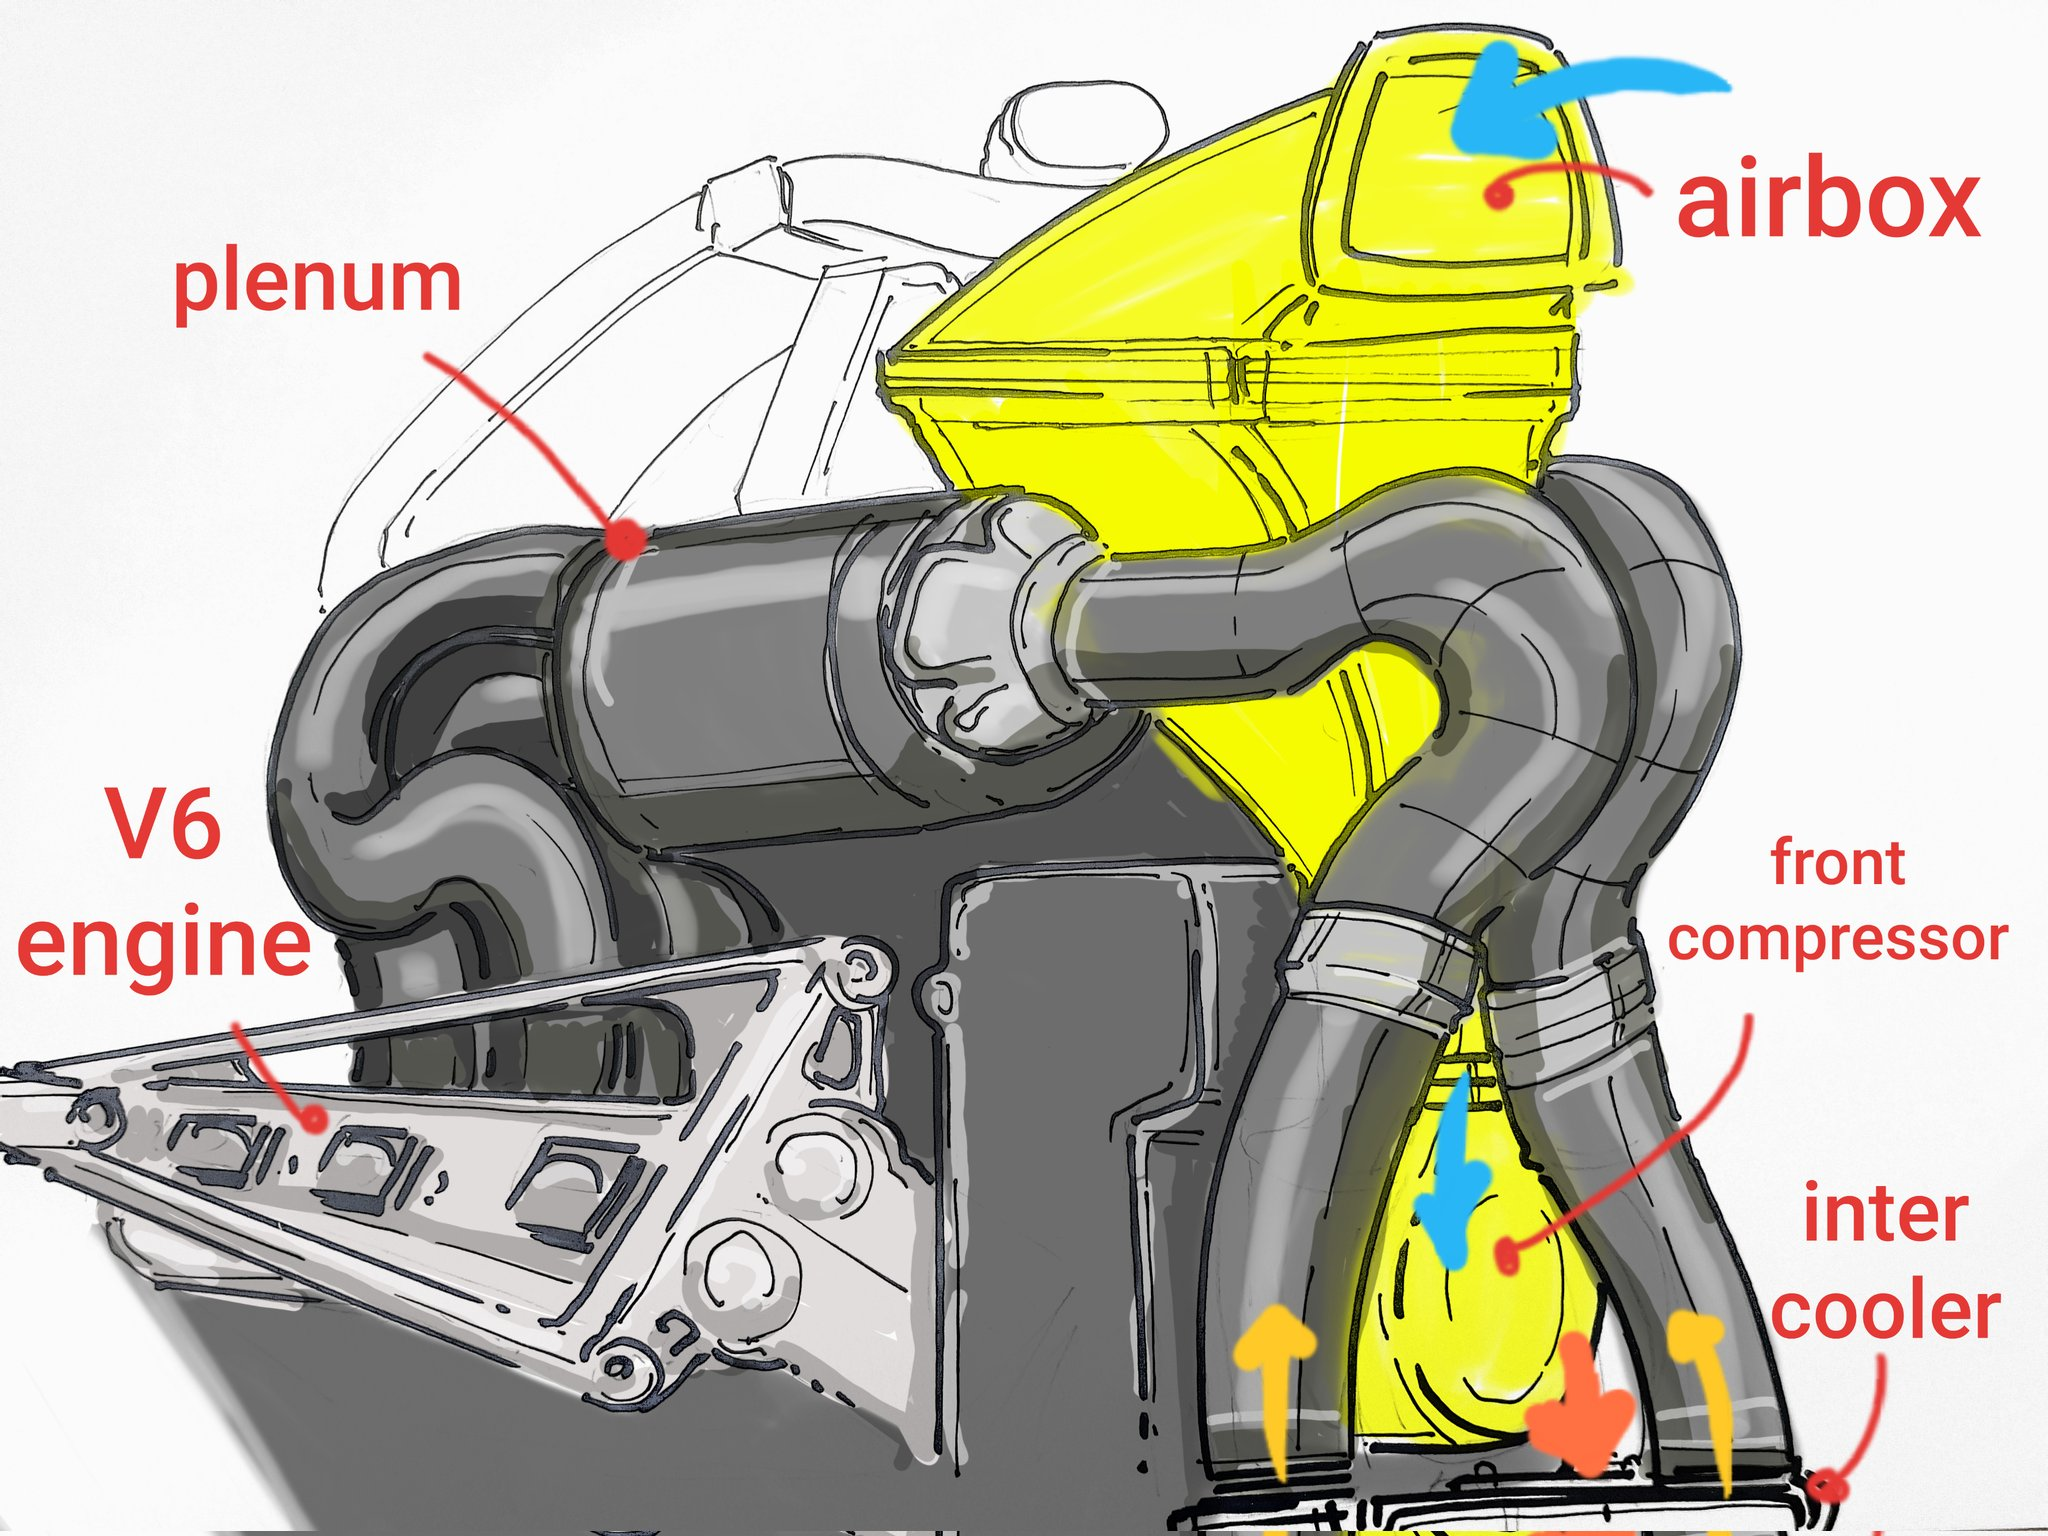
\includegraphics[width=0.8\textwidth]{images/f1-engine.jpg}
    \caption{Proses pembakaran pada ICE}
    \label{fig:Proses pembakaran pada ICE}
\end{figure}

Proses ini juga meningkatkan suhu udara, sehingga udara perlu didinginkan kembali dalam pendingin muatan sebelum dimasukkan ke dalam plenum di bagian atas mesin. \newline

Dari sana, ia melewati enam lubang saluran masuk dan melewati dua katup saluran masuk ke dalam silinder. Di situlah bahan bakar mulai berlaku. \newline

Mesin F1 injeksi langsung, seperti kebanyakan mobil jalan modern, sehingga bahan bakar disuntikkan langsung ke ruang bakar. \newline

Bahan bakar diinjeksikan maksimal 500 bar, yang dibatasi oleh regulasi. Meskipun itu lebih dari yang kita temukan pada mesin bensin injeksi langsung di mobil jalan raya, yang biasanya melihat tekanan hingga 350 bar, ini sebenarnya sedikit lebih sedikit daripada yang mungkin kita temukan di diesel modern, di mana tekanan bahan bakar bisa. mencapai hingga 2.500 bar. \newline

Campuran udara dan bahan bakar dikompresi oleh piston sebelum busi menyalakannya. Kekuatan pembakaran menekan piston, yang terhubung ke poros engkol melalui batang penghubung dan, oleh karena itu, mampu menggerakkan poros engkol. \newline

Saat piston naik kembali, katup buang terbuka untuk melepaskan gas buang dari mesin, sehingga seluruh proses dapat dimulai dari awal lagi – hingga maksimum 15.000 kali setiap menit (atau hingga 250 kali per detik). \newline

Gas buang digunakan untuk menggerakkan roda turbin turbocharger yang pada gilirannya menggerakkan kompresor. Apa yang tersisa kemudian keluar melalui knalpot di bagian belakang mobil, dengan sistem wastegate digunakan untuk mengontrol tekanan selama fase ini.

\subsubsection{Sistem knalpot dan pengaruhnya terhadap suara silinder}

Keluarnya gas buang dimulai setelah pembakaran terjadi. Kemudian, selama langkah buang saat piston bergerak kembali ke atas silinder, katup buang terbuka dan gas yang terbakar dikeluarkan dari ruang bakar. Gas kemudian berjalan ke satu set primer atau header, dengan satu primer per silinder (\textcolor{red}{merah}, \textcolor{purple}{ungu}, \textcolor{blue}{biru}). Tiga primer yang berasal dari masing-masing tepi mesin kemudian bergabung bersama dalam kolektor primer tiga-ke-satu (\textcolor{orange}{orange}) dan kemudian pipa sekunder (\textcolor{yellow}{kuning}). Dua sekunder (satu dari setiap sisi mesin) kemudian masuk ke turbocharger.

\begin{figure}[htbp]
    \centering
    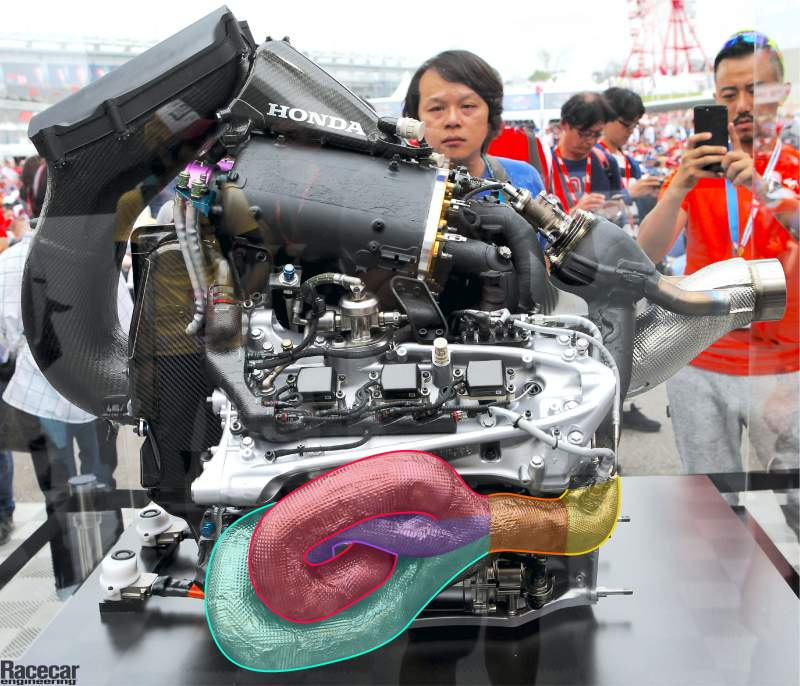
\includegraphics[width=0.7\textwidth]{images/F1-Exhaust-primaries_Honda_RA618H.jpg}
    \caption{Primer (\textcolor{red}{merah}, \textcolor{purple}{ungu}, \textcolor{blue}{biru}), kolektor (\textcolor{orange}{orange}) dan sekunder (\textcolor{yellow}{kuning}) pada \textit{power unit} Honda RA618H 2018}
    \label{fig:The primaries (red, purple, blue), collector (orange) and secondaries (yellow) on the 2018 Honda RA618H power unit}
\end{figure}

Bergantung pada pabrikan mesin, primer, kolektor, dan sekunder dapat menjadi satu bagian dan diintegrasikan ke dalam turbocharger, atau bagian terpisah. Knalpot (\textcolor{blue}{biru}) dari turbocharger kemudian membawa gas buang dari turbo ke bagian belakang mobil. Sementara ada juga wastegate yang mengontrol kecepatan turbo dan terdiri dari satu atau dua pipa wastegate (\textcolor{red}{merah}) yang keluar dari sekunder dan melewati rumah turbin, keluar di bagian belakang mobil.

\begin{figure}[htbp]
    \centering \footnotesize
    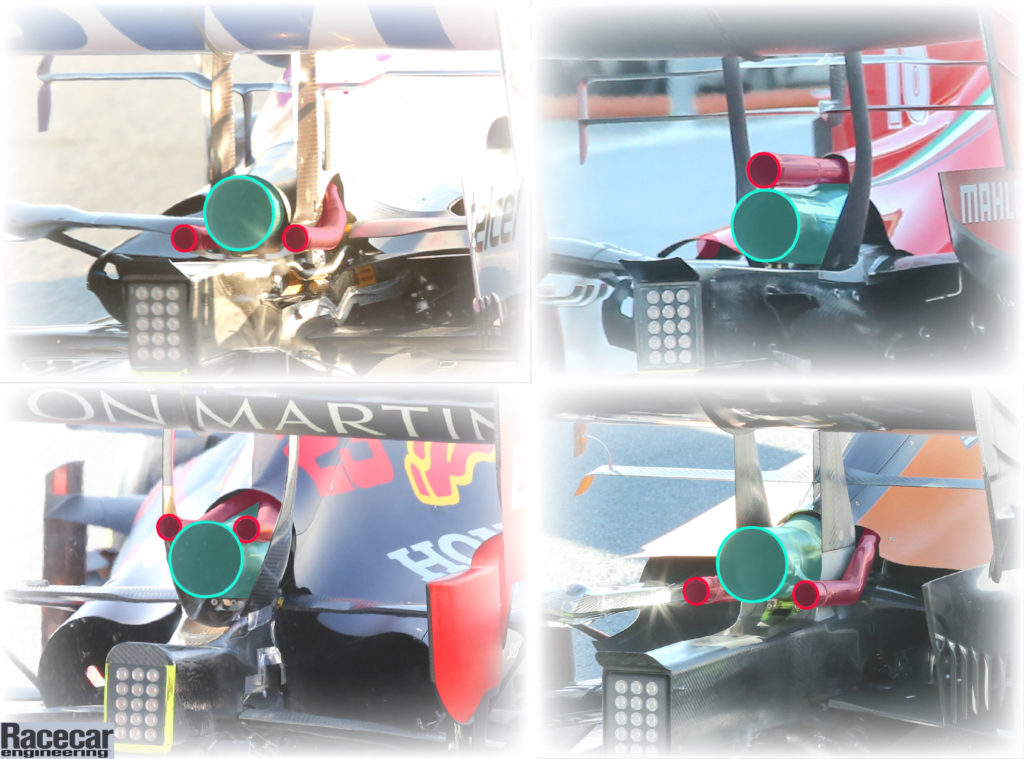
\includegraphics[width=0.7\textwidth]{images/F1-Exhaust-tailpipe-comparison-1024x759.jpg}
    \caption{Tata letak knalpot (\textcolor{blue}{biru}) dan wastegate (\textcolor{red}{merah}) dari empat \textit{power unit} yang berbeda. Kiri atas: Mercedes (Racing Point RP20). Kanan atas: Ferrari SF1000. Kiri bawah: Honda (Red Bull RB16). Kanan bawah: Renault (McLaren MCL35) (Sumber : https://www.racecar-engineering.com) }
    \label{fig:The tailpipe (blue) and wastegate (red) layouts of the four different power units. Top left: Mercedes (Racing Point RP20). Top right: Ferrari SF1000. Bottom left: Honda (Red Bull RB16). Bottom right: Renault (McLaren MCL35)}
\end{figure}

Meskipun konsep sistem pembuangan tampak relatif sederhana, ada banyak ilmu di balik parameter seperti panjang pipa, diameter, dan tata letak yang dapat dimanipulasi untuk menyetel torsi dan pita daya mesin.

\subsubsection{Karakteristik suara silinder pada mesin F1}

Mesin F1 dapat memiliki berbagai konfigurasi jumlah silinder, seperti V6TH (Turbo Hybrid), V8, V10, atau V12, tergantung pada peraturan yang berlaku pada saat tersebut. Umumnya, mesin dengan jumlah silinder yang lebih besar, seperti V10 atau V12, cenderung menghasilkan suara yang lebih berat, dalam hal volume dan kekayaan harmonik. Mesin dengan jumlah silinder yang lebih sedikit, seperti V6TH (Turbo Hybrid), cenderung menghasilkan suara yang lebih ringan atau teredam, tetapi dapat mencapai tingkat revolusi mesin yang lebih tinggi dan suara yang lebih tajam.

\subsection{Klasifikasi Suara Menggunakan FFT dan Deep Learning}
\subsubsection{Pengenalan tentang analisis Fourier Transform (FFT)}

TBA

\subsubsection{Penerapan FFT pada analisis suara silinder}

TBA

\subsubsection{Peran Deep Learning dalam klasifikasi suara}

TBA

\newpage